\documentclass{../template/texnote}

\title{\textbf{\capitalisewords{Why the Sky is not the Limit for Astronomy Research?}}}

\begin{document}
    \maketitle \currentdoc{note}
    %<*note>
	\section{Intro}

The sky has attracted the curiosity of the human mind ever since the dawn of civilization and continues to excite us to this day. Our concept of the sky changed drastically during the scientific revolution. From being considered the abode of the Gods, it has become the cosmic laboratory to conduct observations and learn about the universe. 
The scientific revolution was spearheaded by astronomers like Copernicus, Galileo, and Newton amongst countless others, who were intrigued by the mysteries of the sky and dared to find answers. In this article, we shall try to answer some of the following questions. What is astronomy? What is the state of research in astronomy? How has astronomical research benefited the broader scientific community? Does research in astronomy have any impact on the life of the common man apart from satisfying his curiosity? Is it still relevant to pursue astronomy research today?

\section{What is Astronomy?}

The dictionary defines it as the study of celestial objects, space, and the physical universe as a whole. You might be tempted to ask what these celestial objects are and why they are so important to study. The objects most familiar to ancient humans were probably the Sun, the moon, and the stars. While stars moved in circular patterns during the night, some of them showed eccentric motions. These wanderers were the planets and they didn't twinkle like the other stars. They were noticed by the ancient civilization like the Babylonians, Greeks and others. In the early 20th century, when Hubble was able to measure the distance to a particular star known as a Cepheid variable (M31\_V1) he found it to be 2.5 million light years away from us. The average distance to most others stars in the night sky is just around 5 light years. Thus we came to know of galaxies of stars beyond our own. These galaxies look like fuzzy objects in the sky compared to the pinpricks of light that comes from stars.

With the discovery of ground-based telescopes and telescopes sent to space on satellites, today the sky has turned into a cosmic zoo. Several types of objects have since been discovered. There are Nebulae that are the cradles of stars. Neutron stars and black holes, which are the favorites of science fiction writers. Brown dwarfs and white dwarfs, Quasars and pulsars. The red giants and Cepheid variables and much more. Then there are several astrophysical phenomena like solar and lunar eclipses, red moons and aurora, supernovae and GRBs, solar flares, comets, meteors, and meteorites. 
% \section{Fields of Research in Astronomy}
Several fields are currently under study in astrophysics. These include space weather prediction, search for near-Earth objects, planetary explorations, stellar evolution, gravitational waves, dark matter, and dark energy amongst others. 

But is it worthwhile to devote time and resources to studying such things when we have more important problems to solve here on Earth?  Why do people spend huge amounts of money and time on such frivolous pursuits? In order to understand this, let us look at the history of astronomy and see what lessons it has to teach us. 

\begin{figure}
    \centering
    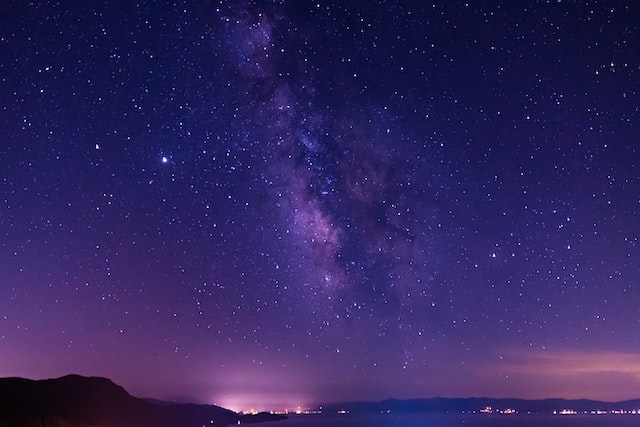
\includegraphics[scale=0.6]{Linn/tyler-clemmensen-DQ_KYf1LF6E-unsplash.jpg}
    \caption{The milky way galaxy as seen over Lake Tahoe (Image Credit: 
Tyler Clemmensen on Unsplash.com)}
    \label{fig:milkyway}
\end{figure}


% \begin{figure}
% \begin{tabular}{cc}
%   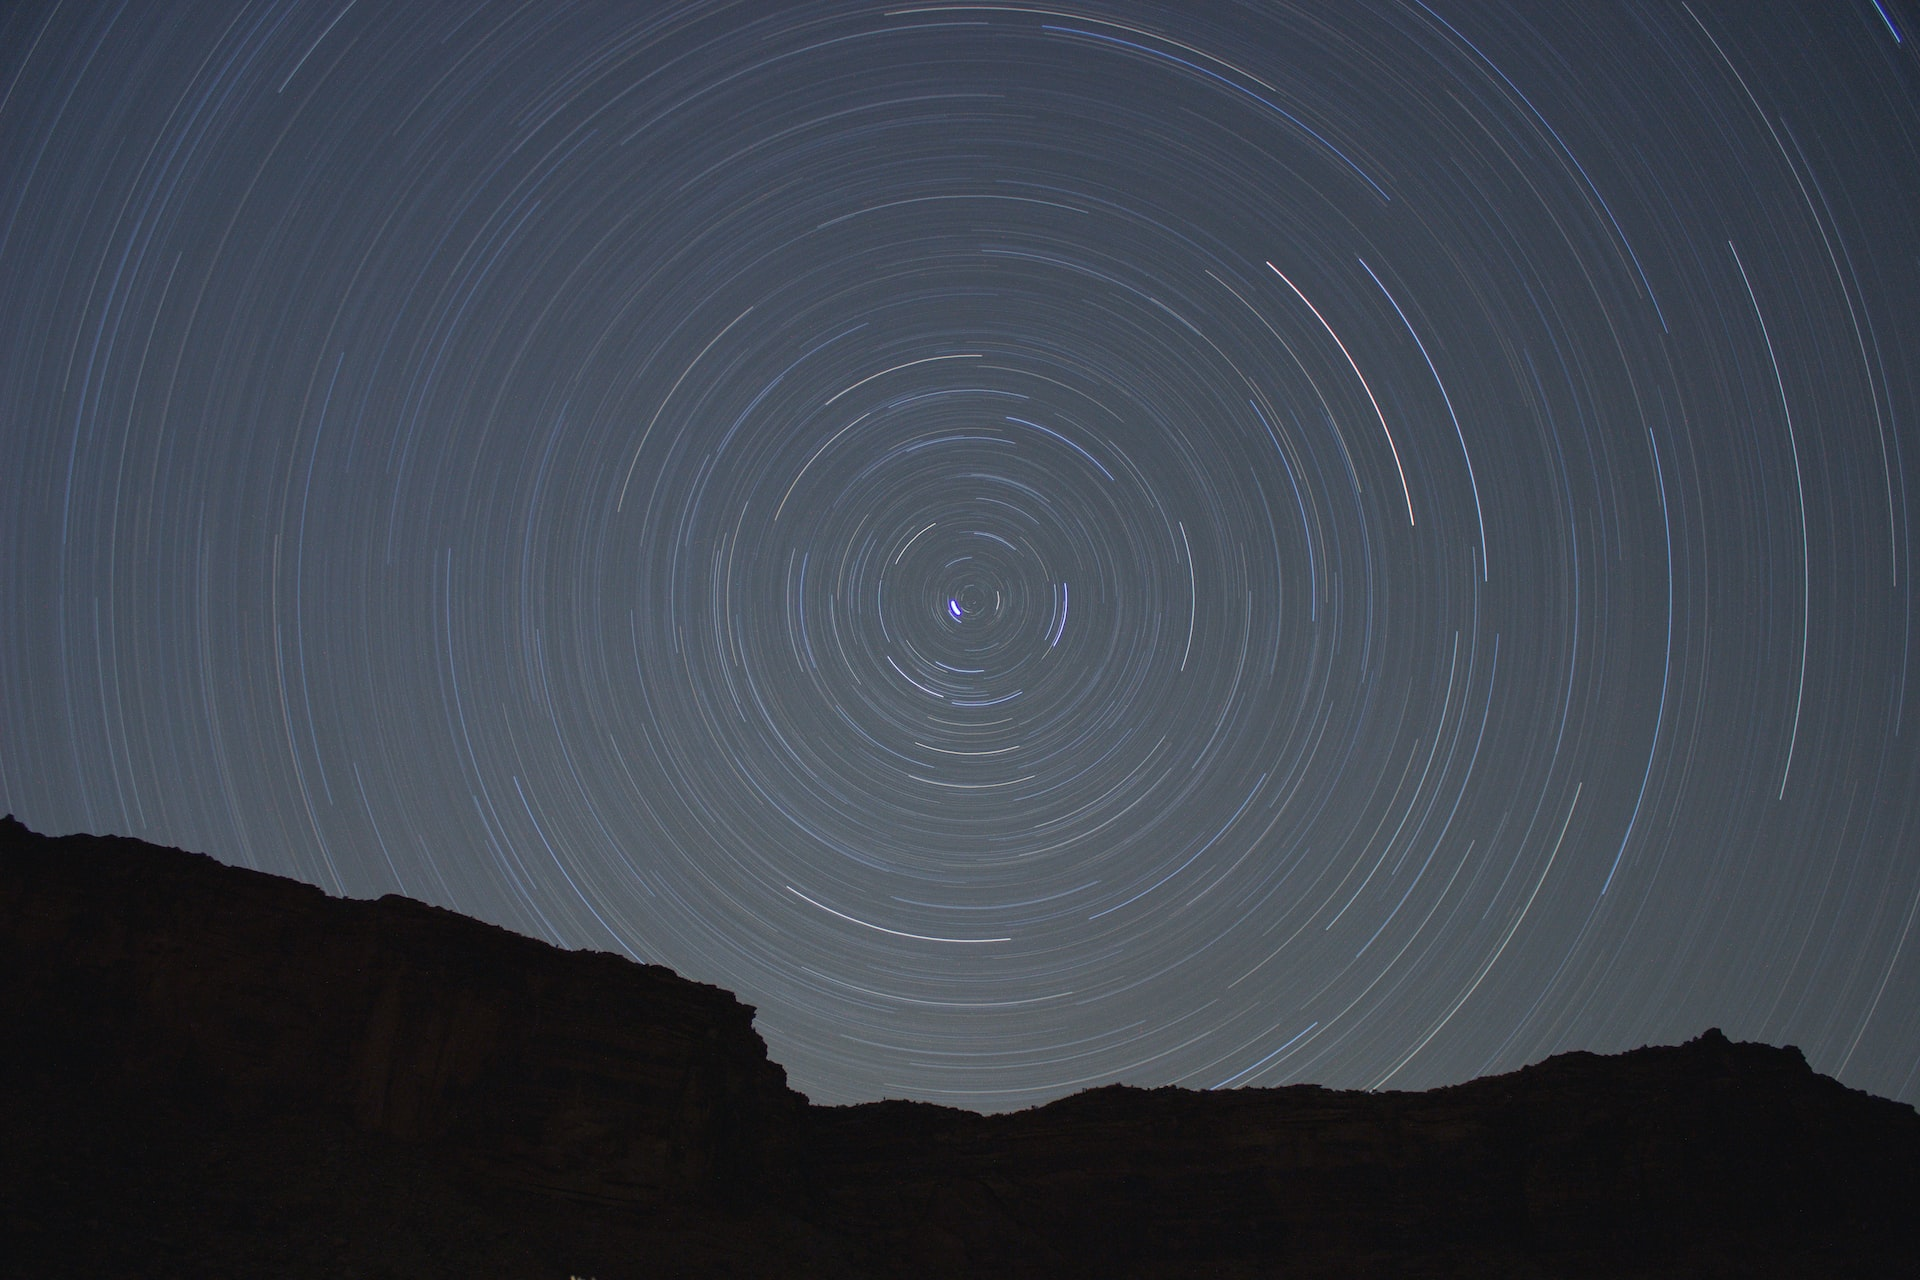
\includegraphics[width=0.5\textwidth]{Linn/michael-hull-UdvXJ95Yqt8-unsplash.jpg} &   
%   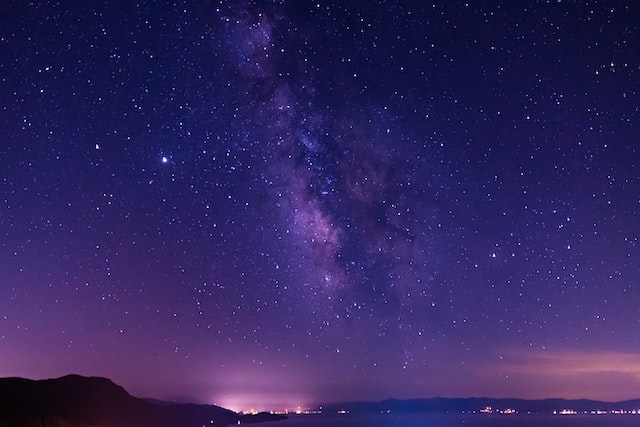
\includegraphics[width=0.5\textwidth]{Linn/tyler-clemmensen-DQ_KYf1LF6E-unsplash.jpg} \\
% \end{tabular}
% \caption{On the left,Star trails captured using long exposure photography. (Image Credit: Michael Hull on Unsplash.com ).
% On the right,
% The milky way galaxy as seen over Lake Tahoe (Image Courtesy: 
% Tyler Clemmensen on Unsplash.com)
% }
% \label{fig:Ancient}
% \end{figure}


\begin{figure}
    \centering
    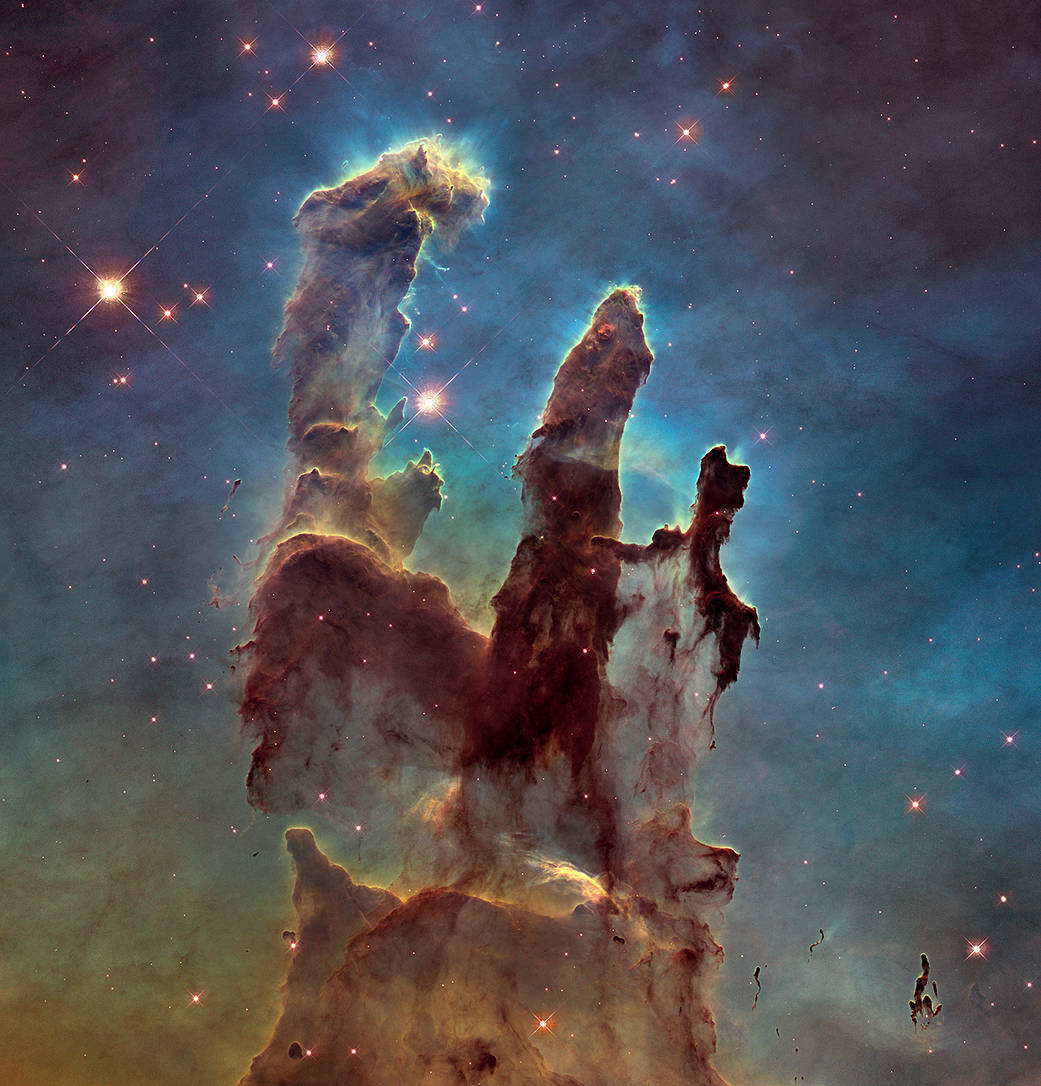
\includegraphics[scale=.4]{Linn/pillars_of_creation.jpg}
    \caption{These towering tendrils of cosmic dust and gas sit at the heart of M16, or the Eagle Nebula. The aptly named Pillars of Creation, featured in this stunning Hubble image, are part of an active star-forming region within the nebula and hide newborn stars in their wispy columns. (Image Credit: NASA, ESA and the Hubble Heritage Team (STScI/AURA))}
    \label{fig:nebulae}
\end{figure}



\section{Astronomy in the Ancient Era}
\begin{figure}
    \centering
    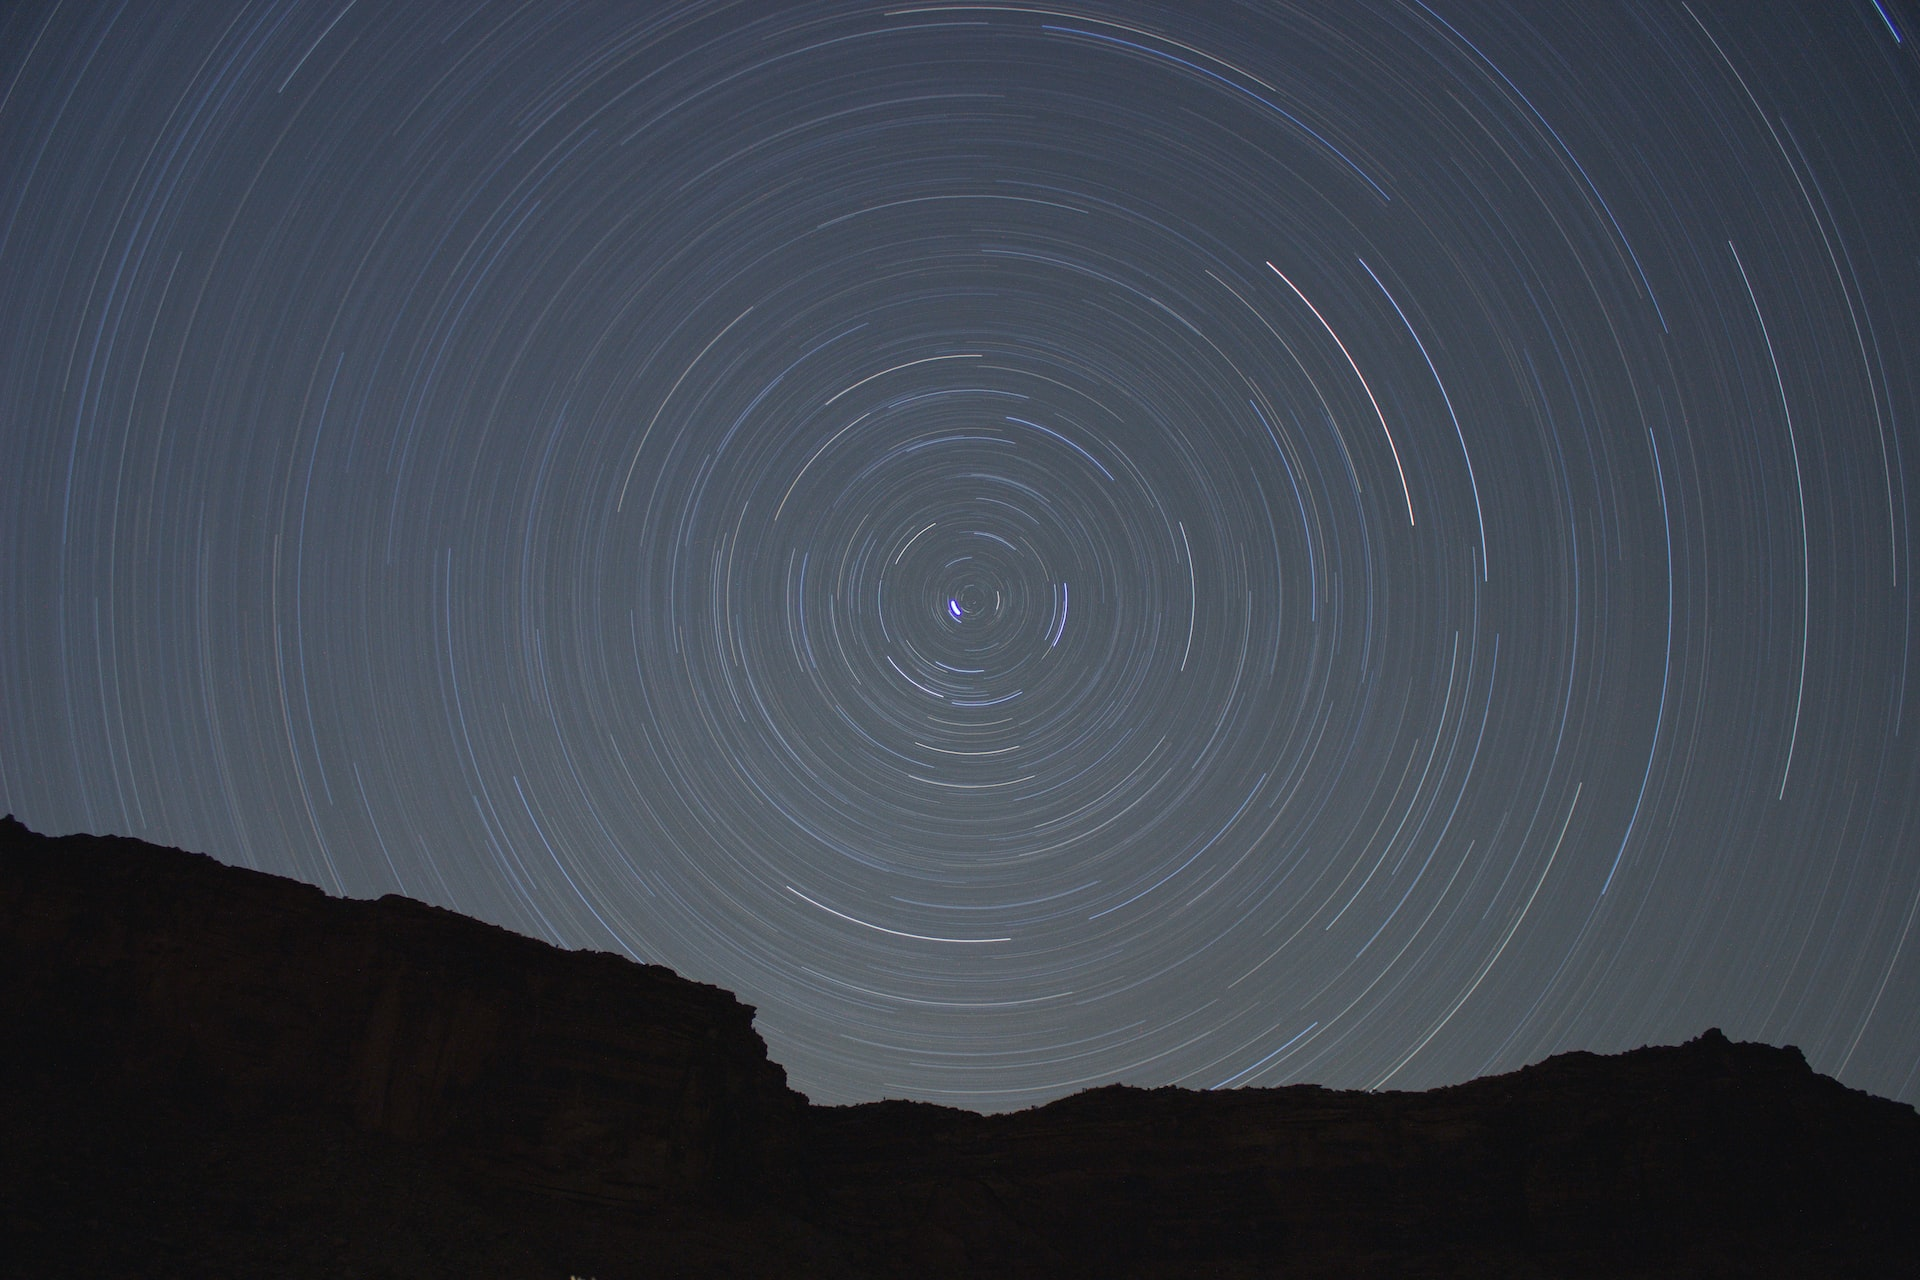
\includegraphics[scale=0.2]{Linn/michael-hull-UdvXJ95Yqt8-unsplash.jpg}
    \caption{Star trails captured using long exposure photography. (Image Credit: Michael Hull on Unsplash.com)}
    \label{fig:my_label}
\end{figure}

% \begin{figure}
%     \centering
%     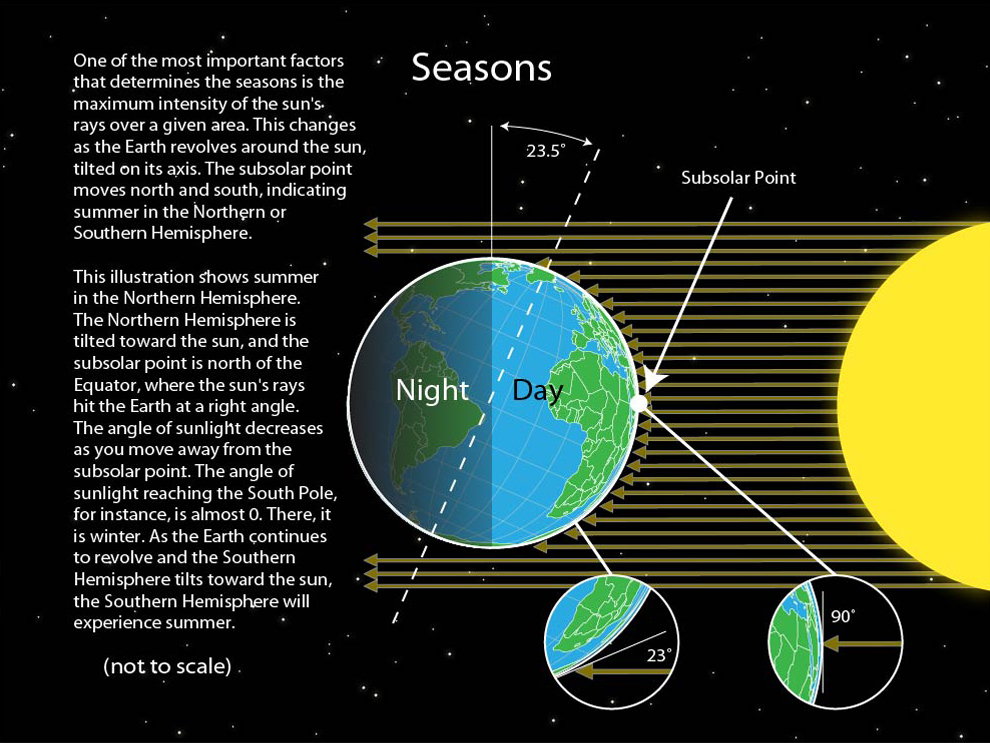
\includegraphics[scale=1.6]{Linn/seasons.jpg}
%     \caption{Formation of the Seasons. (Image Credit: National Geographic)}
%     \label{fig:my_label}
% \end{figure}


\begin{figure}[htbp]
  \centering
  \begin{minipage}[b]{\textwidth}
    \centering
    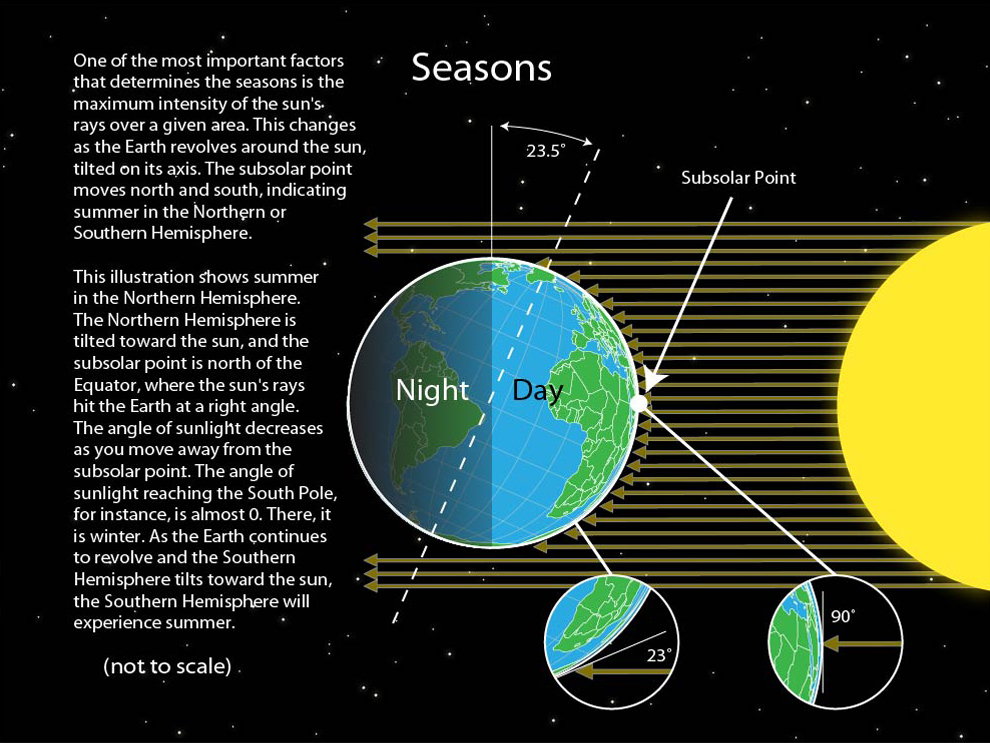
\includegraphics[width=\textwidth]{Linn/seasons.jpg}
    \caption{Formation of the Seasons. (Image Credit: National Geographic)}
    \label{fig:seasons}
  \end{minipage}
  \vspace{0.5cm}

  
  \begin{minipage}[b]{\textwidth}
    \centering
    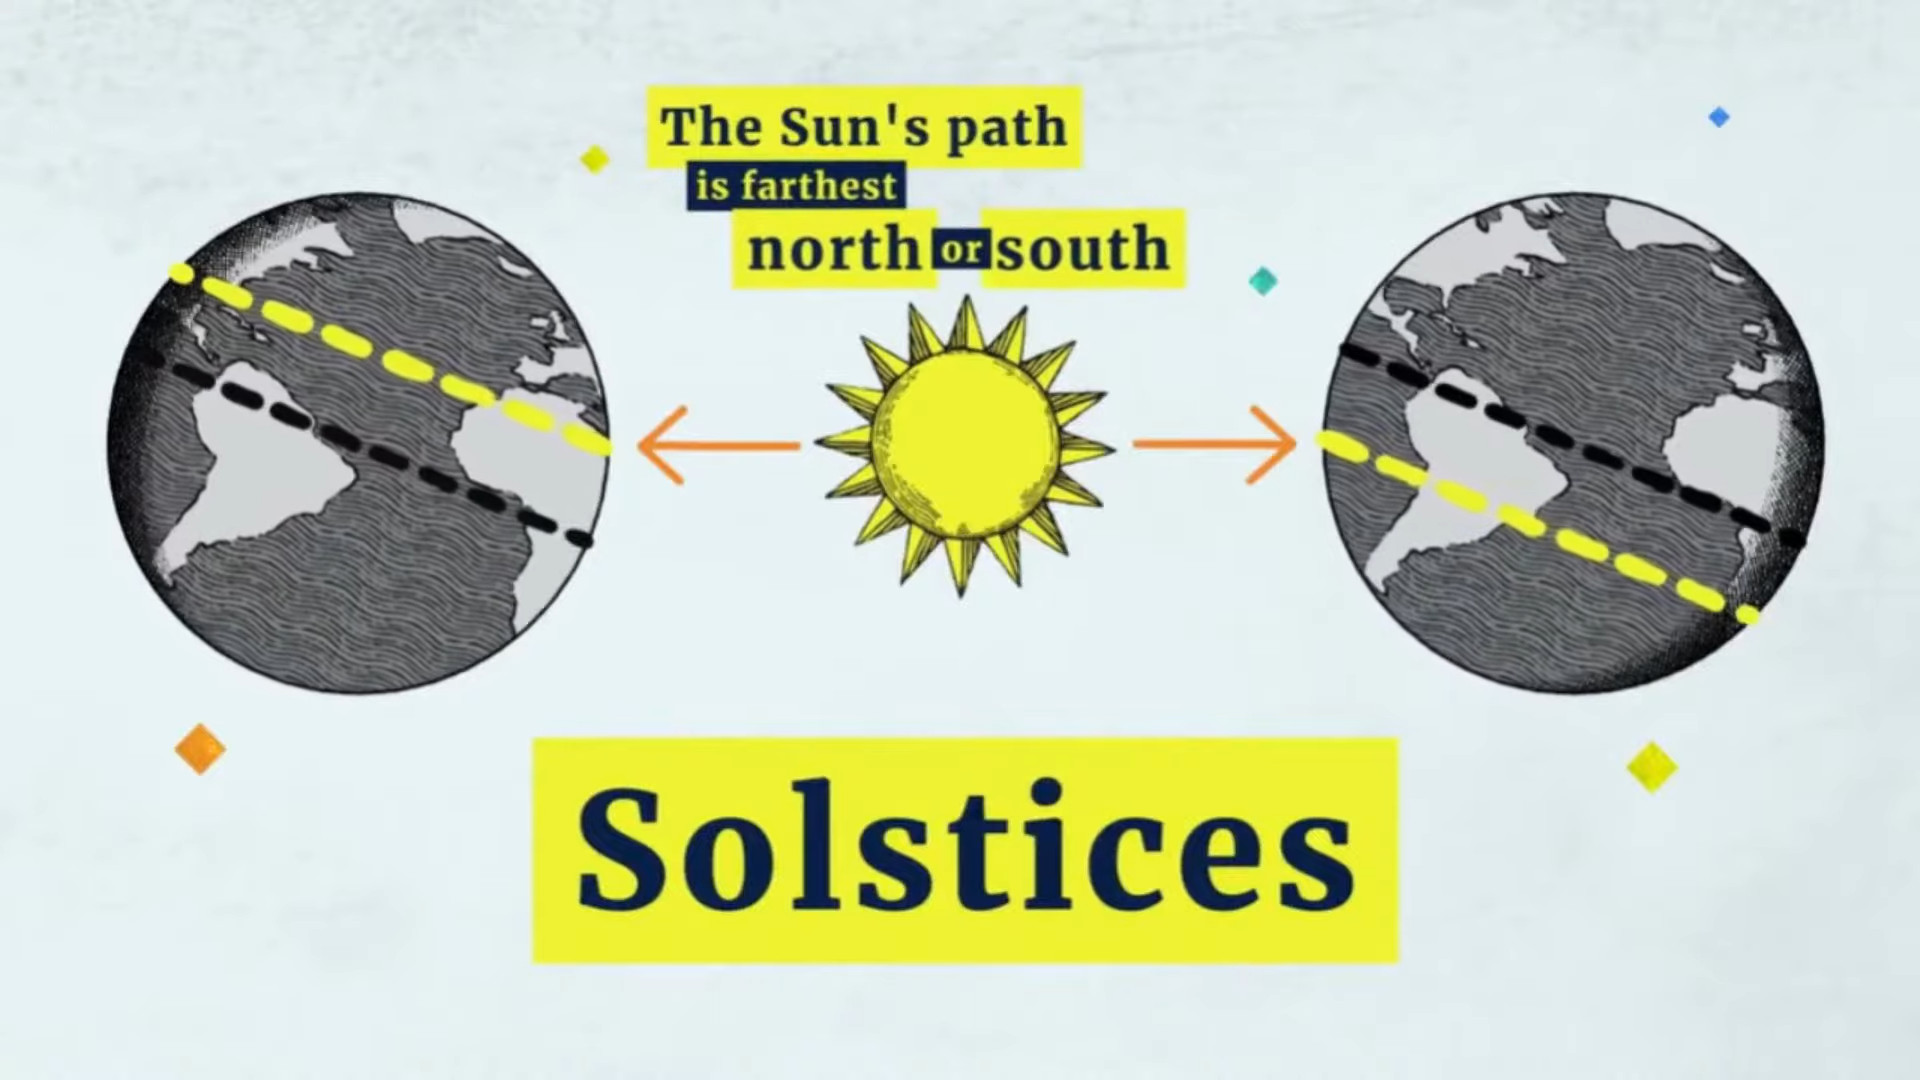
\includegraphics[width=\textwidth]{Linn/solstice.jpg}
      \caption{ Explanation of Solstices. (Image Credit: CosmoVerse Youtube Channel) }
  \label{fig:solstice}
  \end{minipage}
\end{figure}


Astronomy is one of the oldest branches of science and one that has revolutionized Science in many ways. Man's curiosity about the sky probably started in pre-historic times. His pattern-seeking brain sought answers to things like the motion of the stars, the waxing and waning of the moon, and the freckles on the lunar surface. Answers were scarce to come by and he had to make do with stories and fables. But those who persisted in their investigations did not do so in vain. Observations of the sky led them to discover a star that never changed its position in the sky. This was the pole star or polaris that always pointed north. In hindsight now we know the motion of the stars to be caused due to the rotation of the Earth about its axis. Hence a star that is directly above the north pole would scarcely move. This helped them to navigate the vast oceans especially during the night when the Sun is no longer there to provide directions. Observations of the lunar cycles, the solstices, and equinoxes helped to keep time by creating calendars and helped them decide when to plant their crops. Because of the tilt of the Earth's axis the Northern hemisphere appears to point maximally towards the Sun once during the year and away from the Sun at the end of the year. The subsolar point is the place which receives the maximum intensity of the Sun's light. This point moves North to South throughout the year through an angle of 47\textdegree. Solstices designate the point in the Earth's orbit around the Sun when the Sun's path in the sky or the subsolar point is the farthest North or South from the equator. The duration of day and night varies both with the latitude of a place and the point where you have reached in the Earth's orbit around the Sun. But at any point on the Earth's surface the Solstices are marked by the days that have longest and shortest durations. 


\section{The Age of Scientific Revolution}

\begin{figure}
    \centering
    %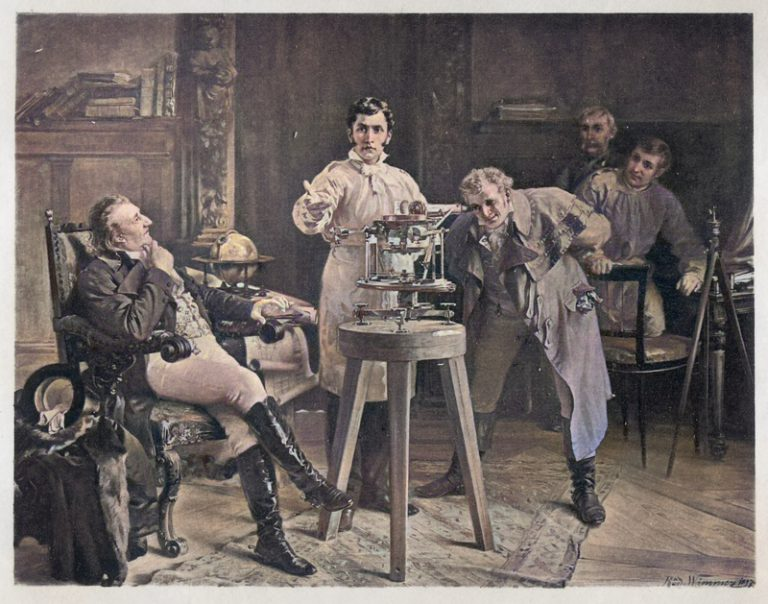
\includegraphics[scale=0.45]{Linn/Fraunhofer_spectroscope-768x604.jpeg}
    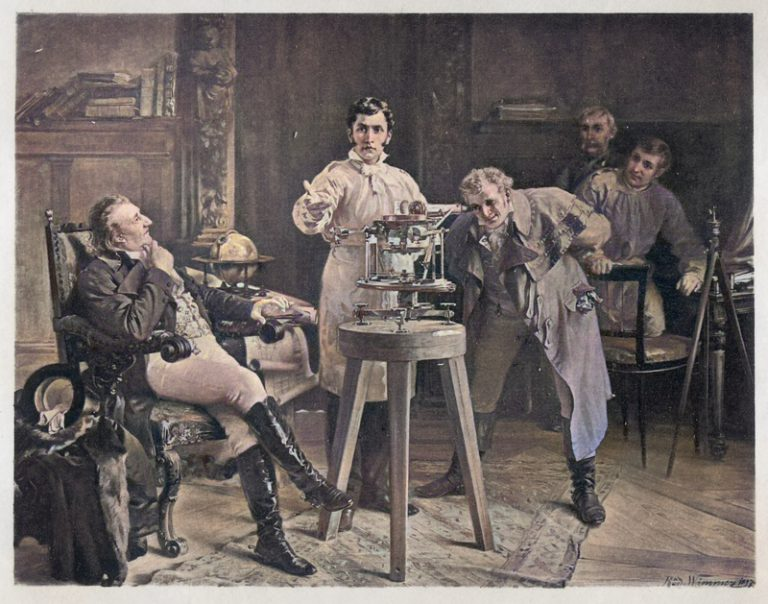
\includegraphics[width=0.8\textwidth]{Linn/Fraunhofer_spectroscope-768x604.jpeg}
    \caption{Joseph von Fraunhofer (1778-1826) demonstrating the spectroscope}
    \label{fig:spectroscope}
\end{figure}

The giants that spearheaded the scientific revolution like Aristotle, Copernicus, Galileo, Kepler, and Newton were all astronomers. Science as we know it today emerged from the efforts of these pioneers. The Copernican hypothesis of a heliocentric universe was nothing short of an Earth-shattering event when it came to be confirmed through the observations of Galileo and others. Issac Newton framed his laws of motion drawing heavily upon Kepler's work on the laws of planetary motion. 

Astronomy contributed heavily to the development of science in the centuries that followed. Fraunhoffer who tried to analyze the Solar spectrum found dark lines in it. Scientists later found that these lines could be used to identify the chemical composition of stars. The revolutionary technique of spectroscopy was born. Using this we came to know that the bright blobs of light in the heavens, the Sun, and the stars are not solid or liquid but made of gas, particularly hydrogen. Today spectroscopy is not only used in astronomy but in other fields such as chemistry, material science, biology, and environmental science. 


% \begin{figure}
% \begin{tabular}{cc}
%   % 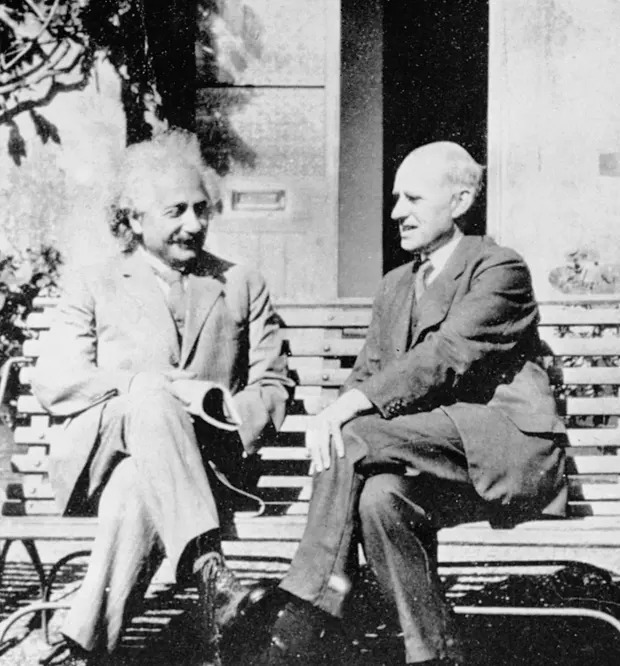
\includegraphics[height=3.4in,width=0.45\textwidth]{Linn/4252.jpg} &
%   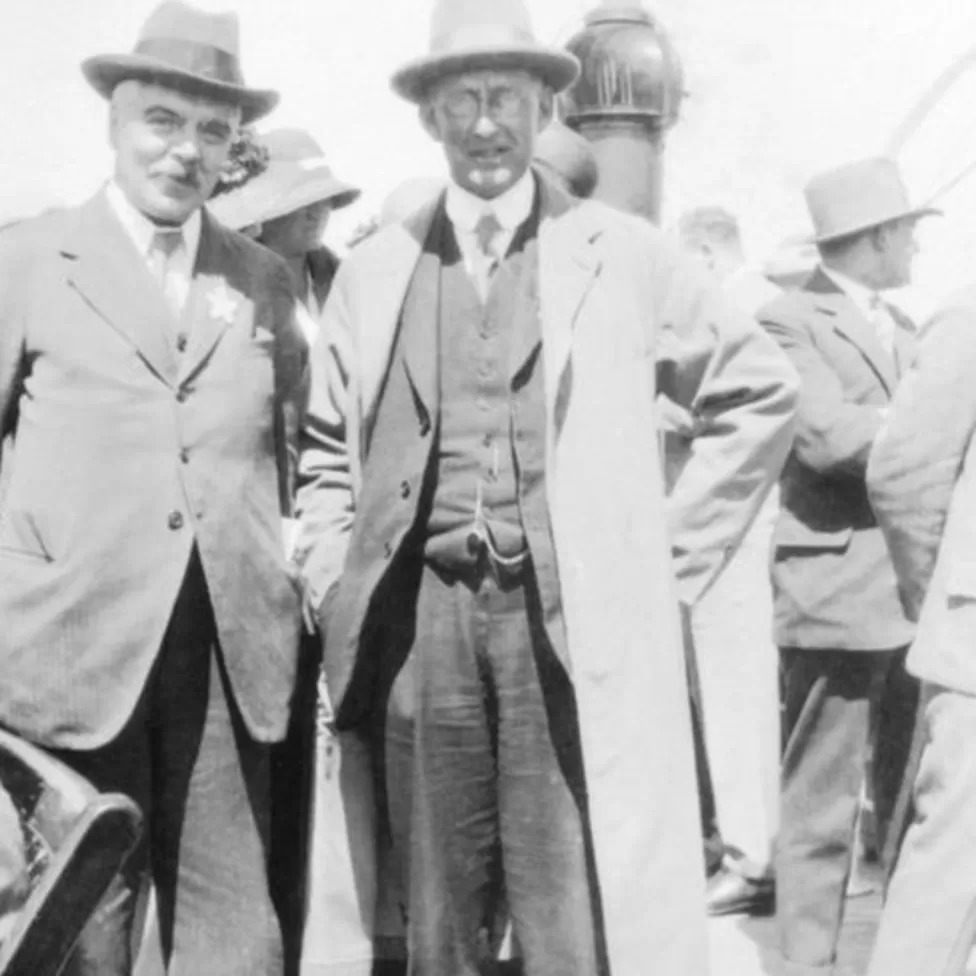
\includegraphics[height=3.4in,width=0.55\textwidth]{Linn/_107065827_e1f50415-b714-4846-bc6a-4b93a1c756b5.jpg}
%       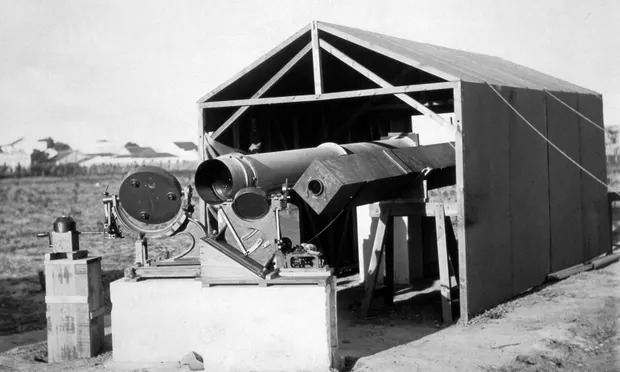
\includegraphics[height=3.4in,width=0.55\textwidth]{Linn/3504.jpg} 
% \end{tabular}
% \caption{On the Left, Einstein and Eddington at the University of Cambridge Observatory, in 1930. (Image Credit: Royal Astronomical Society/Science Photo Library). On the right, Instruments used to observe the 1919 total solar eclipse, Sobral, Brazil. (Image Credit: Science \& Society Picture Library/SSPL via Getty Images))
% }
% \label{fig:Einstein_and_Eddington}
% \end{figure}

% \begin{figure}
% \centering
% 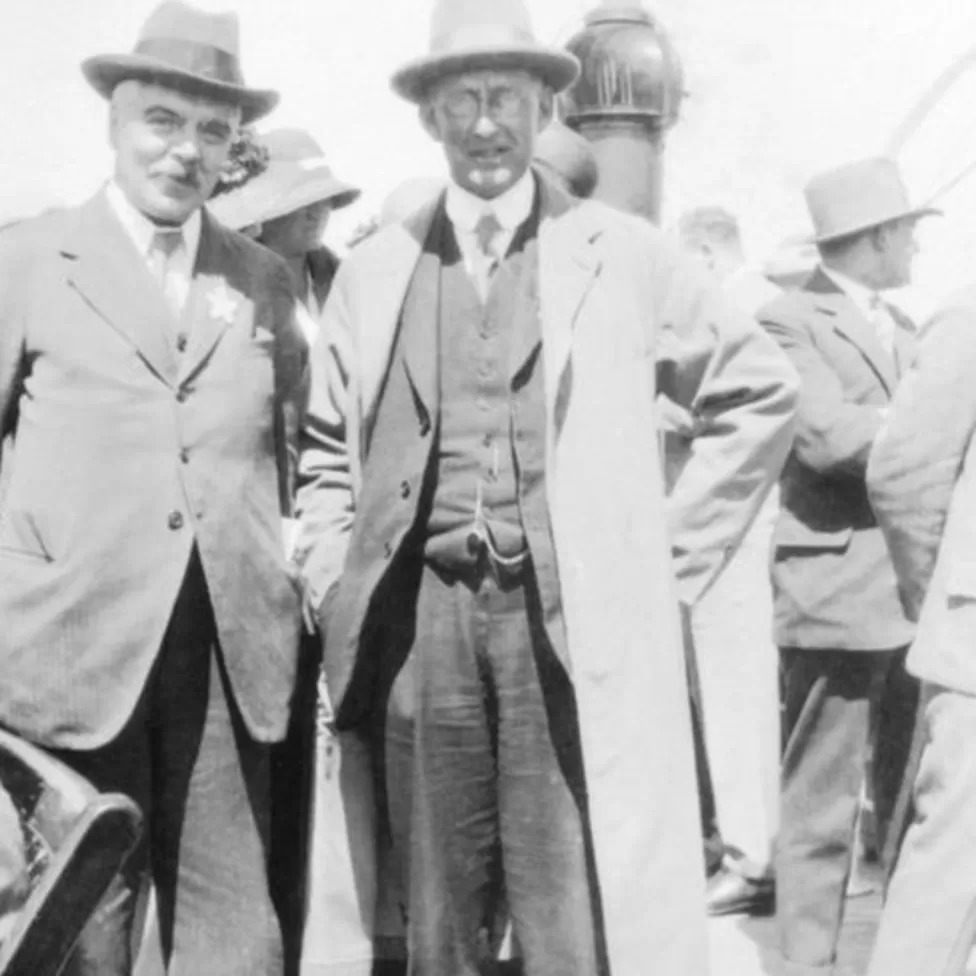
\includegraphics[scale=0.25]{Linn/_107065827_e1f50415-b714-4846-bc6a-4b93a1c756b5.jpg}
% \caption{Frank Dyson (left) and Arthur Eddington (right) during the Solar eclipse experiment that propelled Einstein to fame. (Image Credit: AIP Emilio Segrè Visual Archives, W. F. Meggers Collection).
% }
% \label{fig:Einstein_and_Eddington}
% \end{figure}

% \begin{figure}
%     \centering
%     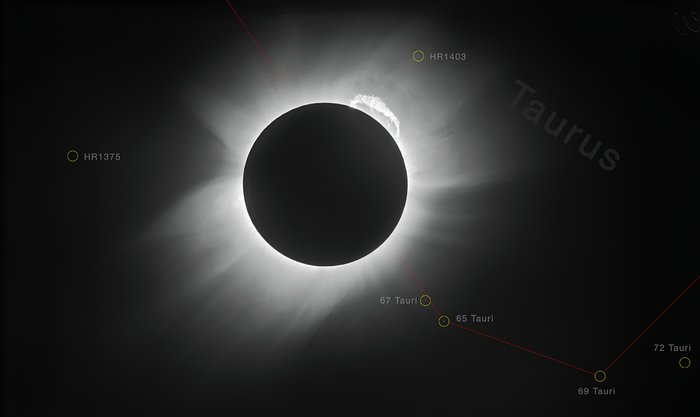
\includegraphics[scale=0.5]{Linn/potw1926a.jpg}
%     \caption{Caption}
%     \label{fig:my_label}
% \end{figure}

% \begin{figure}
%     \centering
%     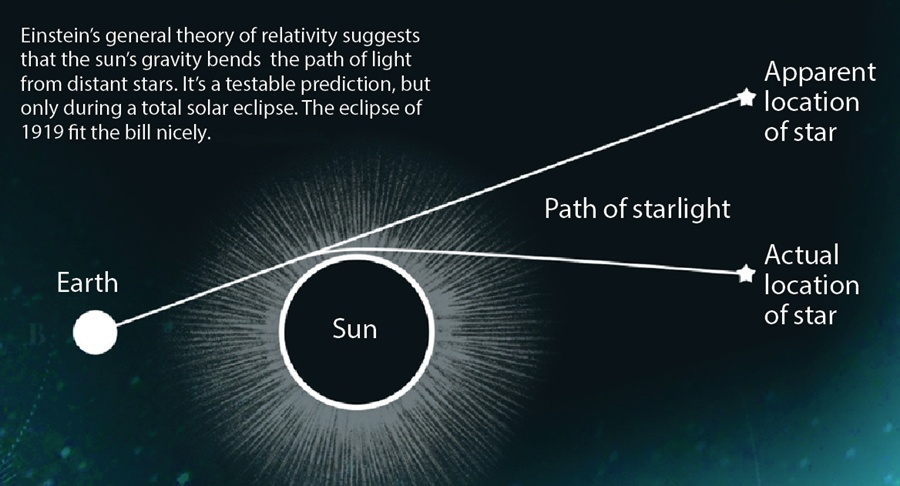
\includegraphics[scale=0.5]{Linn/Star-Positions.jpg}
%     \caption{Caption}
%     \label{fig:my_label}
% \end{figure}

% \begin{figure}
% \begin{tabular}{cc}

%   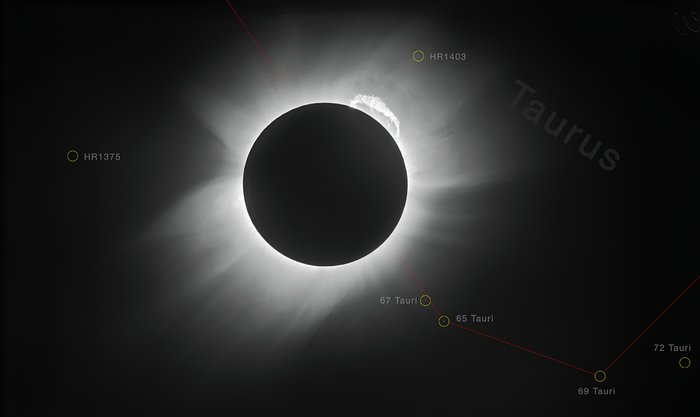
\includegraphics[height=3.4in,width=0.55\textwidth]{Linn/potw1926a.jpg}
%       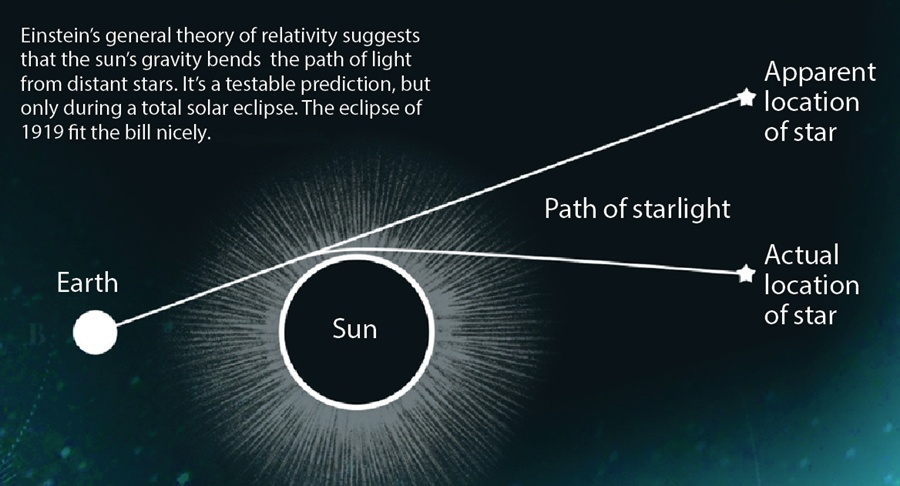
\includegraphics[height=3.4in,width=0.55\textwidth]{Linn/Star-Positions.jpg} 
% \end{tabular}
% \caption{On the Left, Einstein and Eddington at the University of Cambridge Observatory, in 1930. (Image Credit: Royal Astronomical Society/Science Photo Library). On the right, Instruments used to observe the 1919 total solar eclipse, Sobral, Brazil. (Image Credit: Science \& Society Picture Library/SSPL via Getty Images))
% }
% \label{fig:Einstein_and_Eddington}
% \end{figure}

\begin{figure}[htbp]
  \centering
  \begin{minipage}[b]{\textwidth}
    \centering
    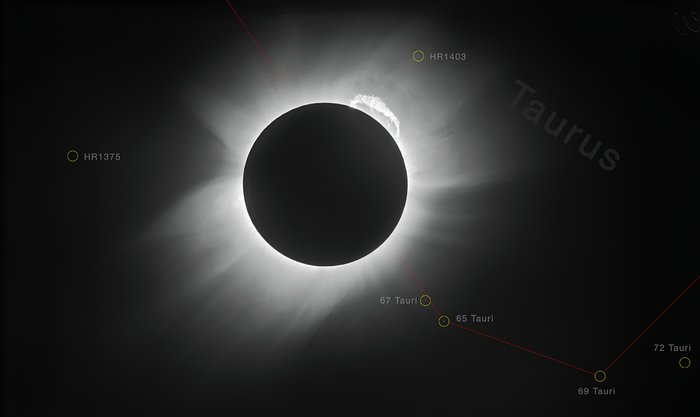
\includegraphics[width=\textwidth]{Linn/potw1926a.jpg}
    \caption{The highest resolution image of the 1919 eclipse. It is the result of applying modern image processing techniques — including image restoration, noise reduction, and removal of artifacts — to the original photographic plate copy. It unveils stunning details in the solar corona, a giant prominence emerging from the upper right part of the Sun, and stars in the constellation of Taurus (The Bull) that were used to confirm general relativity’s predictions.}
    \label{fig:eclipse}
  \end{minipage}
  \vspace{0.5cm}

  
  \begin{minipage}[b]{\textwidth}
    \centering
    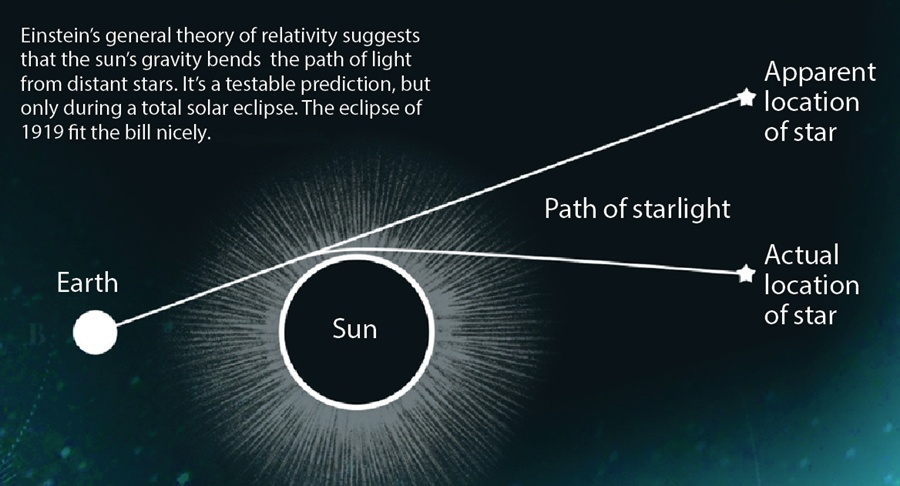
\includegraphics[width=\textwidth]{Linn/Star-Positions.jpg}
    \label{fig:image2}
  \end{minipage}
  \caption{ A diagrammatic sketch of the theory behind the experiment. }
  \label{fig:eclipse_sketch}
\end{figure}




After nuclear physicists unlocked the power of the atom by nuclear fission processes it didn't take them long to identify that the huge source of power in the stars might be from a similar process. We know stars today to be exploding hydrogen bombs that work by the principle of nuclear fusion. 

Astronomy was used to measure the speed of light and also to test the theories of Albert Einstein. Most famously his general relativity theory was tested by Arthur Eddington during the solar eclipse of 1919. Einstein's theory predicts that if light from a star passes very close to a massive object like the Sun, it can bend due to the distortion of space-time. However, when the stars are in the line of sight with the Sun it is not possible to photograph them due to the blinding light of the Sun. The test needed to wait till the next solar eclipse when these stars could be precisely imaged and then compared to images of the same stars viewed from a different vantage point without the Sun in between. The precession of mercury's orbit was also something that could not be explained by Newtonian mechanics but was a natural prediction in Einstein's theory. Many of his other theories are such that they can only be tested by astrophysical observations.  

\section{Astronomy in The Space Race Era}

% \begin{figure}
% \begin{tabular}{cc}
%   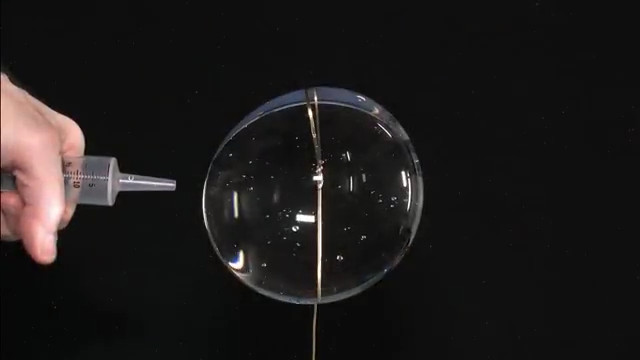
\includegraphics[scale=0.35]{Linn/ScienceofftheSphereAstroPuffsv1.jpg} &
%       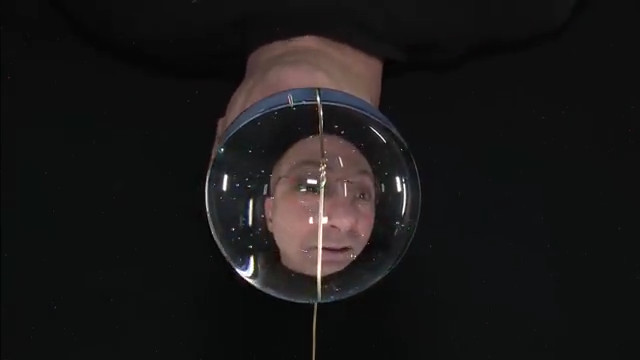
\includegraphics[scale=0.35]{Linn/ScienceofftheSphereAstroPuffsv2.jpg} 
% \end{tabular}
% \caption{Water droplet in the zero gravity environment of the ISS forming a lens.
% }
% \label{fig:}
% \end{figure}
\begin{figure}
    \centering
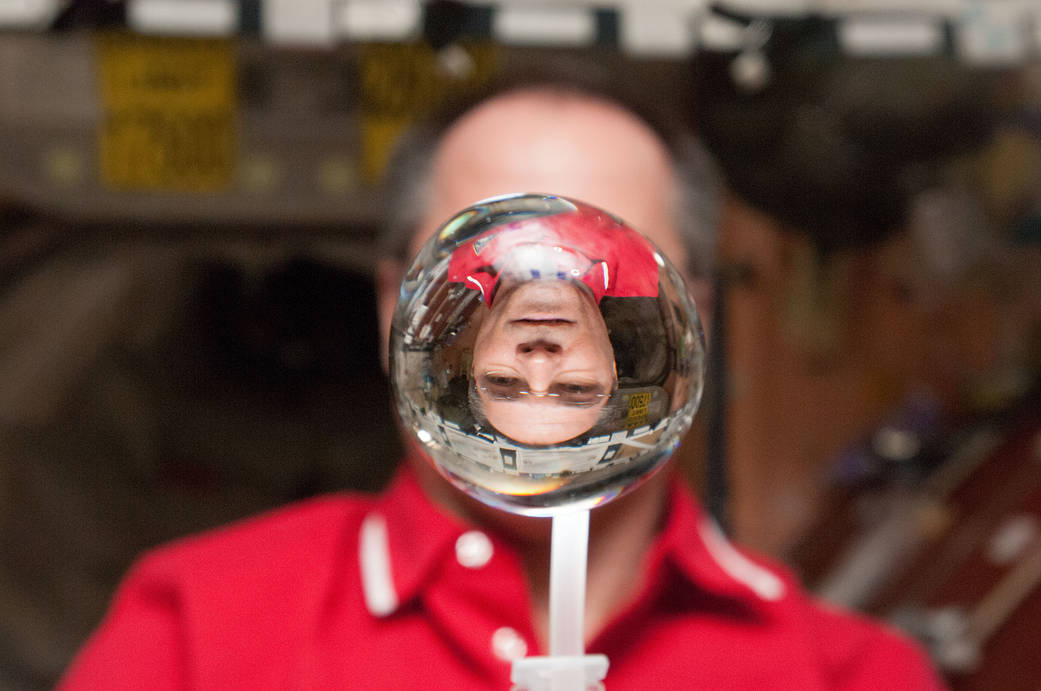
\includegraphics[scale=1.5]
{Linn/723520main_8413732347_ceb0cc9a40_o-full_full.jpg}
    \caption{NASA astronaut Kevin Ford, watches a water bubble float freely between him and the camera, showing his image refracted, in the Unity node of the International Space Station.(Image Credit: NASA)}
    \label{fig:iss}
\end{figure}


The first man-made satellite sent to orbit around the Earth had no other purpose other than to demonstrate Soviet superiority. However, this event marked the beginning of the space race in which the United States and the Soviet Union constantly competed with each other. All of humanity was to benefit from this race. Soon the potential of satellites was explored for studying and forecasting weather, and extreme events such as hurricanes and tornadoes. They were used for data transmission and defense purposes. The GPS system that is heavily used today was developed as part of the military applications of satellites. The moon that our ancestors could only look at and weave stories about were touched upon by a man in the year 1969. 

Space provides scientists with unique possibilities for conducting research. This includes providing an environment with long-term exposure to microgravity, radiation, and vacuum conditions. It also  provides a unique vantage point for observing the universe. In space, the blurring effects of the atmosphere that makes stars twinkle and spread out are absent. The sky can be observed in its full glory in frequencies that would normally be blocked by our atmosphere such as UV, X-rays, and Gamma Rays. 

NASA the premier organization that conducts space and astronomy research has a web page dedicated to spin-off technologies. These are technologies that have found commercial use in our daily lives. The page now lists almost 2000 such technologies and includes some of the most important technologies of our age.  A few of these include solar cell, water filtration based on activated charcoal, freeze-dried food, infra-red ear thermometers, portable kidney dialysis machines, satellite television, advanced prosthetics, scratch-resistant lenses, and memory foams. 




\section{The Impact of Astronomy Research}

Analyzing the historical evidence it becomes clear that the importance of astronomy research to the world cannot be overstated. The benefits of astronomy research as in research in  other fundamental sciences come in a multitude of ways most of which are unexpected. It satisfies the curiosity inherent in human beings and opens up the arena for bigger and tougher questions. This pushes the limits of our scientific knowledge and technology and drives the quest for knowledge in several different and related fields. 

Research in astronomy calls for extreme engineering feats and innovation. There is probably a reason why the usage "at an astronomical scale" has become commonplace. Astronomy shows us the coldest possible temperatures in the depths of space to the hottest possible temperatures in the cores of stars and galaxies. The fastest moving things, the most energetic phenomenon in the universe, and the most massive objects in our universe. The countless number of stars in our universe are greater than all the grains of sand on the Earth. The development of technology demanded by astrophysical research drives economic growth as well and leads to an overall improvement in our quality of life. The increased economic growth can further fuel research in astronomy. 

\section{The story behind the GPS and the Wireless Internet}

We saw several examples of how the technology that is often developed for astronomy research has contributed to improvements in several related fields. However, let us take just two different technologies that easily demonstrate its economic and scientific value. The GPS network today is valued at billions of dollars not to say anything about the value of countless lives it has helped save. The cesium atomic clocks abroad every one of these satellites was developed exclusively to test the prediction of Einstein's  theory of relativity which predicted a very small discrepancy between the time shown by a clock on the ground and one that is thousands of miles above it and moving at very high velocities. Without accounting for these relativistic effects, the GPS system would accumulate position errors of several kilometers per day, making it practically useless.

The market for WiFi devices is estimated at hundreds of billions of dollars, not counting the economic transactions expedited by its presence. John O'Sullivan was working on a method to reconstruct the signal of a primordial black hole whose information was smeared out due to the interstellar medium that affected the low-frequency and high-frequency components of the signal differently. He designed a physical chip for doing Fast Fourier Transforms (FFT) that later proved to be helpful when he was asked to work on a new project that pioneered the use of low-power radio signals for wireless internet communication.  Here the issue was with the signals being smeared out due to the reverberations caused by a room's geometry.
\section{Astronomy in the Age of Big Data}

\begin{figure}
    \centering
    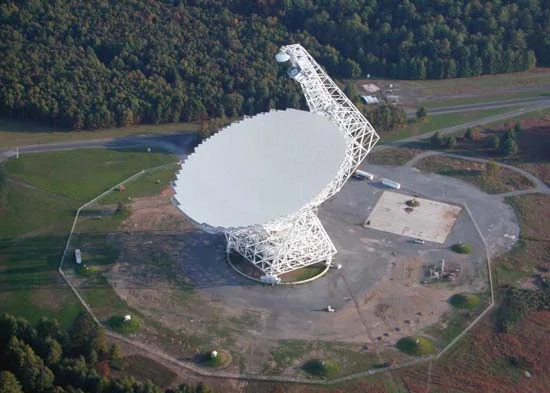
\includegraphics[scale=0.7]{Linn/National-Radio-Astronomy-Observatory-Green-Bank-Telescope.jpg}
    \caption{The National Radio Astronomy Observatory's Green Bank Telescope, Green Bank, West Virginia.(Image Credit-Britannica Encyclopedia)}
    \label{fig:radiotelescope}
\end{figure}

Astronomy has always been at the forefront of technological innovations. Johannes Kepler can very well be considered the first data scientist. After the death of his mentor Tyco Brahe, Kepler inherited a wealth of data that consisted of countless tables of measurements. Tyco Brahe used several pieces of equipment, including quadrants and sextants, to measure the angles between celestial objects and the horizon. He noted the positions, the time of observations, the weather conditions, and the quality of observations. It took Kepler more than six years to formulate his first law of planetary motion from this data. He arrived at the simplest model that fit the observed data, which was an elliptical orbit. 

Today astronomy finds itself among the scientific endeavors that produce and analyze big data. There are robotic telescopes that scan the entire sky multiple times each night taking pictures with short and long exposures. The opening up of new regions of the electromagnetic spectrum including radio, infrared, UV, X-ray and Gamma-ray and the discovery of gravitational waves have opened up the floodgates of data. Add to all of these the digitization of archival data from old photographic plates and we have a field that has the potential for huge discoveries to be made. 

Astronomers have been making use of machine learning and artificial intelligence techniques for solving several challenging problems in astronomy. Most notable among them are the star-galaxy separation problem, the galaxy classification problem, and the detection of signals from gravitational wave data. With several discoveries waiting to be made from existing data and several upcoming surveys already on the drawing board, it is indeed an exciting time for research in astronomy.




\section{References}
\begin{enumerate}
    \item \href{https://www.iau.org/public/themes/astronomy_in_everyday_life/#:~:text=The%20fruits%20of%20scientific%20and,solar%20panels%20and%20Magnetic%20Resonance}{Astronomy in Everyday Life}
    \item \href{http://scihi.org/joseph-fraunhofer-solar-spectrum/}{Joseph von Fraunhofer and the Solar Spectrum}
    \item \href{https://www.amnh.org/learn-teach/curriculum-collections/cosmic-horizons-book/ole-roemer-speed-of-light#:~:text=In%201676%2C%20the%20Danish%20astronomer,eclipses%20of%20Jupiter's%20moon%20Io.}{Ole Roemer and the Speed of Light}
    \item \href{https://www.astronomy.ohio-state.edu/nahar.1/papers/astronomy.magazine.may12.pdf}{What has astronomy done for you lately?}
    \item \href{https://spinoff.nasa.gov/}{NASA Spinoffs}
    \item \href{https://www.bbc.com/news/science-environment-48369980}{The man who made Einstein world-famous}
    \item \href{https://www.eso.org/public/images/potw1926a/}{Highest resolution image of the 1919 solar eclipse}
    \item \href{https://phys.org/news/2015-02-stars.html}{Do stars move?}
    \item \href{https://education.nationalgeographic.org/resource/season/}{Seasons}
\end{enumerate}
    %</note>
    \printbibliography
\end{document}
